\documentclass[12pt]{IEEEtran}

\usepackage{color,soul}
\usepackage{tikz}
\usetikzlibrary{shapes.geometric, arrows, shapes.arrows, decorations.markings, calc}
\usepackage{pgfplots}
\usepackage{listings}
\usepackage{color} %red, green, blue, yellow, cyan, magenta, black, white
\definecolor{mygreen}{RGB}{28,172,0} % color values Red, Green, Blue
\definecolor{mylilas}{RGB}{170,55,241}
\usepackage[english]{babel}
\usepackage{graphicx}
\usepackage{subcaption}
\usepackage{hyperref}
\usepackage{cite}
\usepackage[utf8]{inputenc}
\usepackage{hyperref}

\hypersetup{
    colorlinks=true,
    linkcolor=blue,
    filecolor=magenta,      
    urlcolor=magenta,
}

\urlstyle{same}


\begin{document}
\title{{European University of Lefke} \\ [0.9cm] {Faculty of Engineering} \\ [0.9cm] {Digital Signals Processing EE464} \\ [0.9cm]{Lab report 1}}
\author{\Large \textbf{By: Aimen Zelaci} \\ [0.4cm] \textbf{std-number: 
174553}}
\maketitle

\begin{tikzpicture}[remember picture,overlay]
   \node[anchor=north west,inner sep=0pt] at (current page.north west)
              {
\includegraphics[scale=0.2]{logo.jpg}};
\end{tikzpicture}
\section{Report structure}
This report is organised as follows: an introduction which describes the problem at hand, a theoretical approach to the problem, experimental results that contains the theoretical part results together with the MATLAB implementation, and Finally a conclusion to the results that have been attained.

\section{Introduction}
In the previous coursework we have been requested to implement a type I, 4th-order, linear phase, FIR (Finite Impulse Response) filter, having the following desired impulse response:\\
\[h_{d}[n] = \frac{sin((\frac{\pi}{4}) \times (n - \frac{N}{2}))} {\pi \times (n - \frac{N}{2})} . . . (1)\] \\
Where $N$ is the order of the filter, in this case $N = 4$.\\
The required stopband attenuation is $50 dB$.\\
As a part of this implementation, we were to find and sketch the impulse response $h[n]$, using the window method. Moreover, the transfer function of the digital filter at hand and its block diagram. Finally, we were to discuss the stability of the system based on the previous results.

\section{Theoretical approach}
The first step to tackle this design is to choose a suitable window. With $ 50 dB$ stopband attenuation required, the Hamming window is appropriate as it has $53 dB$ stopband attenuation. Next, to find the requested impulse response we have to multiply both the desired impulse response and the window together:\\
\[h[n] = h_{d}[n] \times w[n] . . . (2)\] \\
Where:\\
\[w[n] = 0.54 - 0.46cos(\frac{2 \pi n}{N}) . . . (3)\]\\
and at $n = \frac{N}{2}$; $h_{d}[n] = \frac{\omega_{c}}{\pi} = 0.25$, such that $\omega_{c} = \frac{\pi}{4}$ is the cutoff frequency.\\
(3) will result in a hamming window symmetrical about $x = \frac{N}{2}$. Thus perfectly containing (1) in the window, since (1) is already shifted by $\frac{N}{2}$ to make the desired impulse response \textbf{causal}.
Now, that we can calculate $h[n]$ using equation (3), we can easily determine the $z-transfer function$, as follows:
\[H(z) = \sum_{n=0}^{4} h[n]z^{-n} . . . (4)\]
To get a proper transfer function which has a denominator and a numerator we multiply (4) by $\frac{z^{4}}{z^{4}}$. (4) shows that the poles of a FIR filter are centred on the origin of the z-plane, thus implying the fact that this system is \textbf{stable}, as the following equation demonstrates:

\[H(z) = \frac{b_{0} + b_{1}z + b_{2}z^{2} + b_{3}z^{3} + b_{4}z^{4}}{z^{4}}...(5)\]

\section{Experimental Results}
As we shall see in this section, equation (3) results in a low pass filter with a cutoff frequency $\omega_{c} = \frac{\pi}{4}$. Therefore, we have used the pre-built MATLAB $fir1$ with the default argument "low pass". The coressponding MATLAB code can be found at \nameref{sec:A}. 

Next, I plotted the resulted impulse response functions in Figure 1. As can be seen, the two responses are different, though they both characterize a linear phase, type I, low pass filter. The reason is that the MATLAB function $fir1$ uses \textbf{the least-squared method} to approximate $h_{d}[n]$. The source code for $fir1$ can be found here: \url{http://read.pudn.com/downloads48/sourcecode/math/163974/fir1.m__.htm}

To sum up this section, the plose-zero diagram, the magnitude and phase frequency response are plotted in Figures 2 and 3 respectively. 

These figures have been obtained using the output impulse response of the $fir1$ function, however, similar results have been obtained when using the theoretical approach with slight difference in the magnitude response and similar linear phase response.
The pole-zero diagram is obtained by employing the coefficients of strictly speaking of (5) (loosely speaking of (4)) as arguments to the MATLAB function $zplane$.

Figure 2 clearly shows that all of the poles of the system are inside the unit circle in the $z-plane$, therefore, implying what we have said earlier that an FIR filter is always stable (regardless of the implementation adopted).

\begin{figure}
   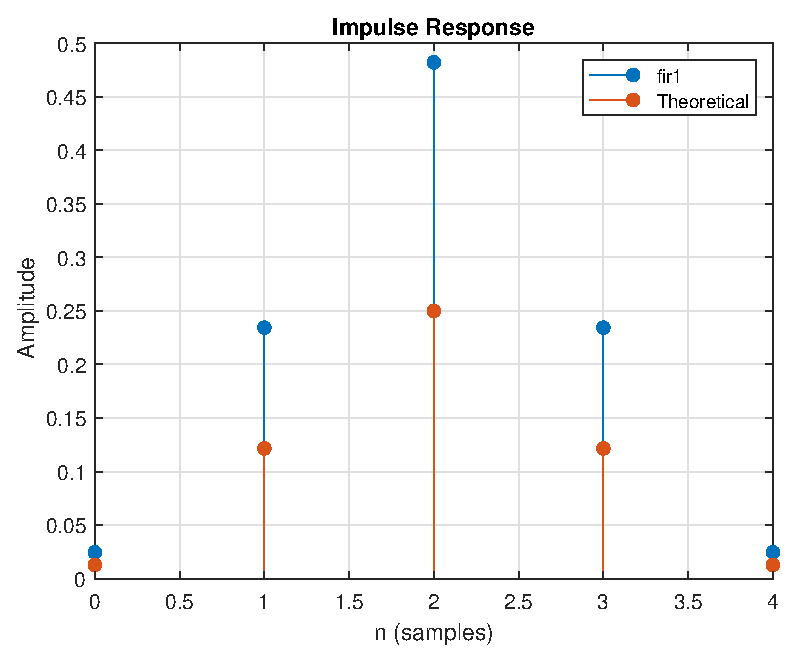
\includegraphics[scale=0.6]{impl.eps}
   \caption{The impulse response functions of both the theoretical approach and the $fir1$ function}
\end{figure}
\begin{figure}
   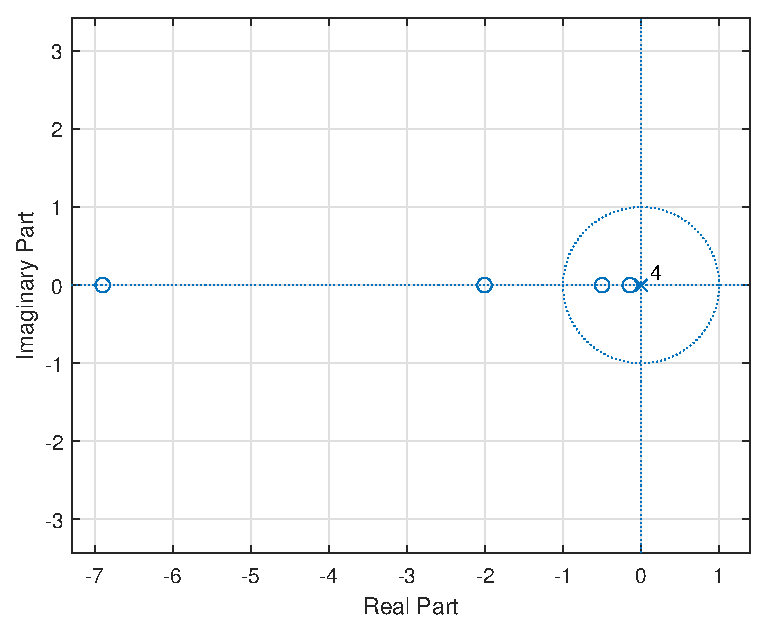
\includegraphics[scale=0.6]{zplane.eps}
   \caption{The pole-zero diagram of the filter (The $Z$-plane)}
\end{figure}  
\begin{figure}
   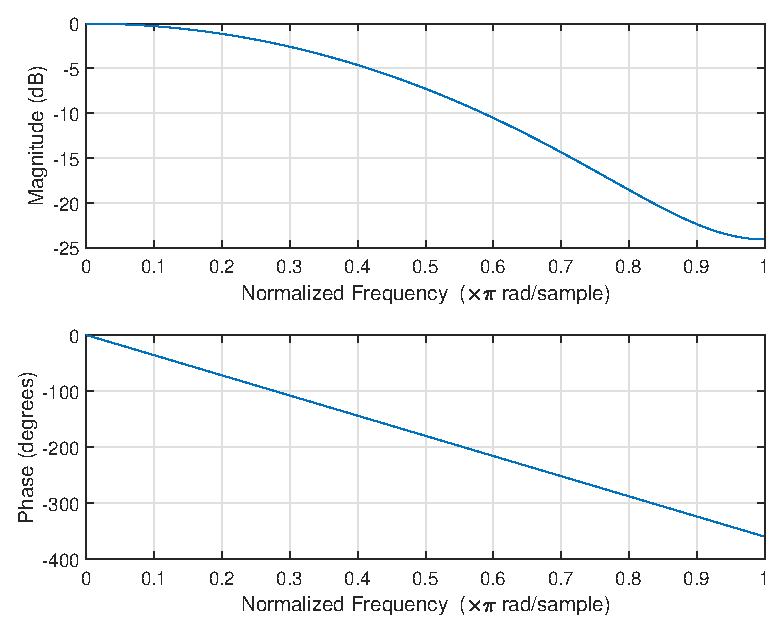
\includegraphics[scale=0.6]{magphse.eps}
   \caption{The magnitude and phase response of the filter}
\end{figure}  

\section{Conclusion}
In this work, we designed a linear phase type I (low pass) filter, employing both the theoretical approach and the pre built MATLAB function $fir1$. Both methods resulted in a different low pass filter due to the fact that $fir1$ function uses the \textbf{linear-squared} method to calculate the desired impulse response. Furthermore, results have shown that both approaches produce identical pole-zero diagrams, therefore concluding that a FIR system is always stable. Finally, both approaches resulted in the same desired linear phase response. 

\section{Appendix A}
\label{sec:A}

\lstset{language=Matlab,%
    %basicstyle=\color{red},
    breaklines=true,%
    morekeywords={matlab2tikz},
    keywordstyle=\color{blue},%
    morekeywords=[2]{1}, keywordstyle=[2]{\color{black}},
    identifierstyle=\color{black},%
    stringstyle=\color{mylilas},
    commentstyle=\color{mygreen},%
    showstringspaces=false,%without this there will be a symbol in the places where there is a space
    numbers=left,%
    numberstyle={\tiny \color{black}},% size of the numbers
    numbersep=9pt, % this defines how far the numbers are from the text
    emph=[1]{for,end,break},emphstyle=[1]\color{red}, %some words to emphasise
    %emph=[2]{word1,word2}, emphstyle=[2]{style},    
}


\section*{Matlab Code}

\lstinputlisting{code.m}
\end{document}